\documentclass[a4paper,10pt]{report}

\def\packagepath{../../../../../preambule}   % path du package principal
\usepackage{\packagepath/preambule}    % utilisation du fichier de configuration

\def\level{BTS }              % Classe
\def\course{CIEL 1}           % Matière
\def\eval{Intégration}          % Titre de l'évaluation

\def\visibleornot{visible}    % visible or invisible
\def\documentpath{./Sources_Latex}
\def\date{C107 - TP2 }
\renewcommand{\arraystretch}{1}  % Ecart dans les tableaux

\def\ptsexoA{0}
\def\ptsexoB{0}

\def\ptstotal{\ptsexoA+\ptsexoB}

\usepackage{hyperref}

\usetikzlibrary{shapes, arrows, positioning}
\usetikzlibrary{shapes.geometric, arrows, positioning, decorations.pathreplacing}

\tikzstyle{etat} = [draw, rounded corners=15pt, minimum width=2.5cm, minimum height=1.2cm, text centered, font=\bfseries]
\tikzstyle{fleche} = [thick, ->, >=stealth]

\usepackage{float}
\usepackage[T1]{fontenc}

% --- L'INTERRUPTEUR ---
\booltrue{afficheCorrige} % Mettez \boolfalse pour masquer le texte (le cadre reste)
%\boolfalse{afficheCorrige} % Mettez \boolfalse pour masquer le texte (le cadre reste)

% --- LA COMMANDE DE CADRE FIXE ---
% #1: Largeur (ex: \linewidth)
% #2: Hauteur (ex: 3cm)
% #3: Contenu de la correction

%\cadreCorrection{width \linewidth}{cm}{}

\begin{document}





\renewcommand{\labelitemi}{\textbullet}

\pagestyle{DS_FP}
\NomPrenomNote{}


\bigskip

\emph{\textbf{Objectif :} Déterminer la constante de temps d'un signal de décharge sous contraintes géométriques, puis valider l'étude par la dérivation et l'intégration.}

\medskip

%%=============================================================
\textbf{PARTIE A: Détermination expérimentale du paramètre $\tau$}


\medskip

On étudie la tension de décharge d'un composant modélisée par la fonction $f$ définie sur $[0; +\infty[$ par la relation suivante:
\[f(x) = 10\cdot \e^{-x/\tau}\] (où $\tau$ est la constante de temps).
\medskip

Le signal doit respecter la contrainte physique suivante:

\begin{itemize}
    \item À l'instant $x=0$, la tension doit être de 10V, soit $f(0) = 10$.
    \item À l'instant $x=2$, la pente de la tangente à la courbe doit être égale à $-1,84$.
\end{itemize}

\begin{enumerate}
    \item Tracer la courbe de $f$ pour différentes valeurs de $\tau$.\hfill $\square$
    \item Identifier la valeur de $\tau$ qui satisfait les contraintes données.\hfill $\square$
    \cadreCorrection{1}{1}{
$\tau = 2$ satisfait les contraintes, car $f(0) = 10$ et $f'(2) = -1,84$.
        }
\end{enumerate}

\bigskip

\textbf{PARTIE B: Étude du signal identifié}

\medskip
Utilisez maintenant la valeur trouvée ($\tau = 2$) pour analyser le comportement du signal $f(x) = 10\cdot \e^{-0,5x}$.

\begin{enumerate}
    \item Tracer la courbe de $f$ et observer son comportement.\hfill $\square$
    \item Affichez la fonction dérivée $f'$ \hfill $\square$
    \item Déterminer le signe de $f'$ et en déduire les variations de $f$.\hfill $\square$
    \cadreCorrection{1}{4}{
        \begin{minipage}{0.58\linewidth}
        $f'(x) = -5\cdot \e^{-0,5x}$, qui est toujours négatif pour $x \geq 0$.

        Par conséquent, $f$ est strictement décroissante sur $[0; +\infty[$.
        \end{minipage}\hfill
        \begin{minipage}{0.4\linewidth}
            \begin{tikzpicture}
    \tkzTabInit[lgt=2,espcl=3.5]
    {$x$ / 1, $signe \, f'(x)$ / 1, $var \, f$ / 1}
    {$0$, $+\infty$}
    \tkzTabLine{}
    \tkzTabVar{}
    \end{tikzpicture}
            
        \end{minipage}
    
        }

        
    \item Placer un point $N$ sur la courbe et observer la valeur de $f(N)$ pour différentes positions de $N$. \hfill $\square$
    \item Déplacez le point $N$ vers la droite (grandes valeurs de $x$) et observez la tendance de $f(N)$.\hfill $\square$
    \item Conjecturez la limite de $f(x)$ lorsque $x$ tend vers $+\infty$. \hfill $\square$
    
    \cadreCorrection{1}{3}{
        Lorsque $x$ tend vers $+\infty$, $f(x)$ tend vers 0, car la fonction exponentielle décroît rapidement.

        Cela signifie que la tension de décharge approche de 0V à mesure que le temps passe, ce qui est cohérent avec le comportement attendu d'un signal de décharge.
        }

\end{enumerate}

\bigskip

\pagebreak
\thispagestyle{DS_LP}

\textbf{PARTIE C: Intégration et Valeur Moyenne}

\medskip


On souhaite évaluer la tension moyenne délivrée par le composant sur un intervalle $[a ; b]$.


\begin{enumerate}
    \item Créer les curseurs $a$ et $b$ avec les valeurs initiales $a=0$ et $b=4$. \hfill $\square$
    \item Déterminer graphiquement l'aire sous la courbe de $f$ entre $a$ et $b$ avec la commande \verb|Aire = Intégrale(f, a, b)|. \hfill $\square$
    \cadreCorrection{1}{2}{
        D'après Géogébra, l'aire sous la courbe de $f$ entre $a=0$ et $b=4$ est d'environ $13,53$ unités d'aires.
        }
        
    \item Observer comment l'aire change lorsque vous modifiez les valeurs de $a$ et $b$.\hfill $\square$
    \cadreCorrection{1}{3}{
Lorsque vous augmentez $b$, l'aire sous la courbe de $f$ entre $a$ et $b$ augmente, car vous incluez plus de la courbe. Inversement, lorsque vous augmentez $a$, l'aire diminue, car vous excluez une partie de la courbe.

        }
    \item Calculer l'aire sous la courbe de $f$ entre $a=0$ et $b=4$ à l'aide de l'intégrale.\hfill $\square$
    \cadreCorrection{1}{3}{
\[A=\int_a^b f(x) \, dx = \int_0^4 10\cdot \e^{-0,5x} \, dx = \left[-20\cdot \e^{-0,5x} \right]_0^4 =  20 \cdot (\e^{-0,5\times 4} - \e^{-0,5\times 0}) = 20 \cdot (1 - \e^{-2}) = 13,53\]

L'aire calculée à l'aide de l'intégrale est d'environ $13,53$ unités d'aires, ce qui correspond à la valeur obtenue graphiquement.


        }
    \item Déterminer la valeur moyenne $\mu$ de la fonction $f$ sur l'intervalle $[a ; b]$.\hfill $\square$
    \cadreCorrection{1}{3}{
\[\mu = \frac{1}{b-a} \int_a^b f(x) \, dx = \frac{1}{4-0} \cdot 13,53 = 3,38\]

La valeur moyenne de la fonction $f$ sur l'intervalle $[0 ; 4]$ est d'environ $3,38$ volts.
        }
    \item Créer un rectangle d'équivalence avec les points \verb|(a,0)|, \verb|(b,0)|,\verb|(b, moy)| et \verb|(a, moy)|. 
    
    Utilisez l'outil \verb|Polygone| pour le colorer.\hfill $\square$
\end{enumerate}

         


\end{document}